\section{Introduction}

The LpzRobots-Simulation is a robot simulation programmed at the university of Leipzig. Its main features
include the \emph{ode\_robots}, which is a 3D robot simulator, that is physically correct, and the so called
\emph{selforg}, that is a framework for controller implementation. \\
The important parts of the software architecture are shown in Figure: \ref{architecture}: \\
\begin{center}
\begin{figure}[h!]
 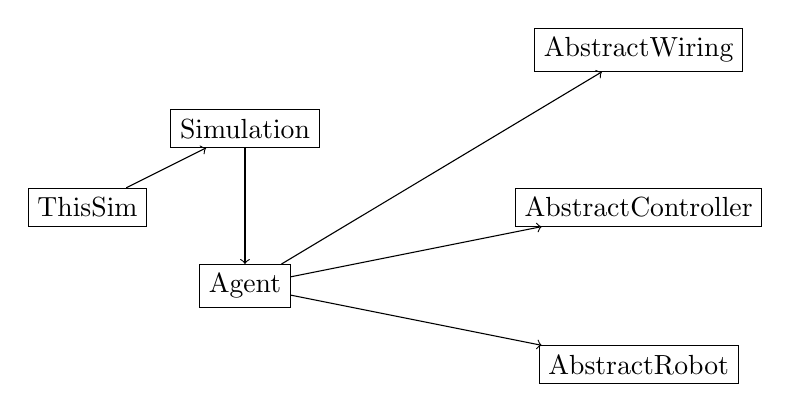
\begin{tikzpicture}
  \node at (0,2) (1) [rectangle,draw] {ThisSim};
  \node at (2,1) (2) [rectangle,draw] {Agent};
  \node at (2,3) (3) [rectangle,draw] {Simulation};
  \node at (7,0) (4) [rectangle,draw] {AbstractRobot};
  \node at (7,2) (5) [rectangle,draw] {AbstractController};
  \node at (7,4) (6) [rectangle,draw] {AbstractWiring};
  \path[->]
	      (3) edge (2)
	      (1) edge (3)
	      (2) edge (4)
	      (2) edge (5)
	      (2) edge (6)
	      ;
 \end{tikzpicture}
 \caption{Software Architecture for LpzRobots and GoRobotos}
 \label{architecture}
\end{figure}
\end{center}
\emph{ThisSim} will, during a simulation, integrate all elements of this very simulation, which means controlling
the environment, the robot, as well as setting initial parameters and plotting or logging data. \\
\emph{Agent} will integrate all elements of an agent by using the shown classes, one can for example add sensory preprocessing
using a child class of \emph{AbstractWiring}. \newline
\begin{center}
  \begin{figure}[h!]
     \begin{tikzpicture}{Simulation}
  \small
  \node at (0,4) (mainE) [rectangle,draw] {\emph{Simulated Environment}: main.cpp};
  \node at (0,6) (amos) [rectangle,draw] {\emph{Simulated Robot}: amonsII.cpp$\backslash$h};

  \node at (0,2) (mainR) [rectangle,draw] {\emph{Real Environment}: main.cpp};
  \node at (0,0) (real) [rectangle,draw] {\emph{Real Robot}: AMOSII\_serial.cpp$\backslash$h};

  \node at (6,5) (amosC) [rectangle,draw] {amosIIcontrol.cpp$\backslash$h};
  \node at (8.5,3.25) (NP) [rectangle,draw] {NeuralProcessing.ccp$\backslash$h};
  \node at (8.5,2.5) (NL) [rectangle,draw] {NeuralLocomotion.cpp$\backslash$h};
  \node at (9,1.5) (CPG) [] {CPG().cpp$\backslash$h};
  \node at (9,1) (PCPG) [] {POSTCPG().cpp$\backslash$h};
  \node at (9,0.5) (PSN) [] {PSN().cpp$\backslash$h};
  \node at (9,0) (VRN) [] {VRN().cpp$\backslash$h};
  \path[->]
	      %(mainE) edge (amos)
	      (mainE) edge (amosC)
	      (mainR) edge (amosC)
	      (mainR) edge (real)
	      (6,2.5) edge (NL)
	      (6,3.25) edge (NP)
	      (7,0) edge (VRN)
	      (7,0.5) edge (PSN)
	      (7,1) edge (PCPG)
	      (7,1.5) edge (CPG)
	      (mainE) edge (amos)
	      ;
  \path[-]
	      (amosC) edge (6,2.5)
	      (7,2.25) edge (7,0)
	      ;


\draw[dashed,color=blue] (-3, 3.5) to (3, 3.5);
\draw[dashed,color=blue] (3, 3.5) to (3, 6.5);
\draw[dashed,color=blue] (3, 6.5) to (-3, 6.5);
\draw[dashed,color=blue] (-3,6.5) to (-3, 3.5);

\draw[dashed,color=red] (-3, -0.5) to (3, -0.5);
\draw[dashed,color=red] (3, -0.5) to (3, 2.5);
\draw[dashed,color=red] (3, 2.5) to (-3, 2.5);
\draw[dashed,color=red] (-3,2.5) to (-3, -0.5);

\draw[dashed,color=mygreen] (4, -0.5) to (11, -0.5);
\draw[dashed,color=mygreen] (11, -0.5) to (11, 6.5);
\draw[dashed,color=mygreen] (11, 6.5) to (4, 6.5);
\draw[dashed,color=mygreen] (4,6.5) to (4, -0.5);
	      

\node at (1.75,1) (sim) [] {\emph{Reality}};
\node at (1.75,5) (reall) [] {\emph{Simulation}};
\node at (7.75,6) (reall) [] {\emph{Control}};
 \end{tikzpicture}
\caption{Need name for this picture}
  \end{figure}


\end{center}
\newpage
For working with the LpzRobots-Simulation, you will need a couple of things:
\begin{enumerate}
 \item A (preferably up-to-date) UNIX-based Operating System (state of the art: Ubuntu 11.10 or Debian 6.0)
 \item The Eclipse-Software combined with the following packages:
      \begin{itemize}
       \item C/C++ SDK
       \item The EGit-Tool-Kit
      \end{itemize}
 \item Access to the Assembla-Repository (contact your supervisor for access)
 \item The setUpGoRobots.zip file (contact your supervisor for the file)
\end{enumerate}